\section{Podstawowe informacje dotyczące przetwarzania obrazów}
\subsection{Podstawowe definicje}
\subsubsection{Piksel}
Piksel jest najmniejszym elementem obrazu cyfrowego. Piksel może określać
\begin{itemize}
\item odcień szarości
\item kolor, wtedy \(f(x, y) = [a(x, y), b(x, y),...]\)\\
  gdzie $a, b,...$ to natężenie poszczególnych barw
\item wskaźnik na element tablicy barw
\end{itemize}
\subsubsection{Obraz cyfrowy}
Obraz cyfrowy definiowany jest jako funkcja:
\begin{gather*}
  f = f(x, y), x = 0,1,2,...,N-1; y = 0,1,2,...,M-1
\end{gather*}
gdzie
\begin{itemize}
\item \(f(x, y)\) - pojedynczy element macierzy, piksel
\item \(M, N\) - szerokość oraz wysokość obrazu
\end{itemize}
Zbiorem wartości dla funkcji obrazu są piksele, dla których każda składowa spełnia warunek:
\begin{gather*}
  f(x, y) \in N
\end{gather*}, gdzie:
\begin{itemize}
\item N - Zbiór liczb naturalnych z przedziału $<0; 2^b>$. Wartość \textit{b} określa liczbę bitów potrzebnych do reprezentacji pojedynczej składowej piksela w obrazie.
\end{itemize}
Przykład obrazu cyfrowego znajduje się na rysunku~\ref{fig:basics_image_color}.
\subsubsection{Obraz cyfrowy jednokanałowy}
Obraz cyfrowy jednokanałowy jest to obraz składający się z pikseli zawierających tylko jedną składową. Zwykle obrazy jednokanałowe wykorzystywane są w celu reprezentacji obrazu w skali szarości. Rysunek~\ref{fig:basics_image_gray} przedstawia jednokanałowy obraz cyfrowy, powstały w wyniku uśrednienia składowych obrazu trójkanałowego.
\subsubsection{Obraz binarny}
Obraz binarny jest to obraz cyfrowy jednokanałowy, którego piksele przyjmują wartości
\begin{gather*}
  f(x, y) = z, z \in \{0, 1\}
\end{gather*}.
Obraz binarny przedstawiony został na rysunku~\ref{fig:basics_image_binary}.
\begin{figure}
  \centering
  \begin{subfigure}[b]{0.45\textwidth}
    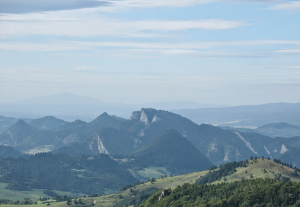
\includegraphics[width=\textwidth]{img/basics-image-color}
    \caption{Trójkanałowy obraz cyfrowy(kolorowy)}
    \label{fig:basics_image_color}
  \end{subfigure}
  ~
  \begin{subfigure}[b]{0.45\textwidth}
    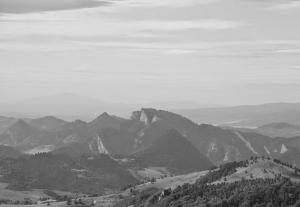
\includegraphics[width=\textwidth]{img/basics-image-gray}
    \caption{Jednokanałowy obraz cyfrowy(skala szarości)}
    \label{fig:basics_image_gray}
  \end{subfigure}
  ~
  \begin{subfigure}[b]{0.45\textwidth}
    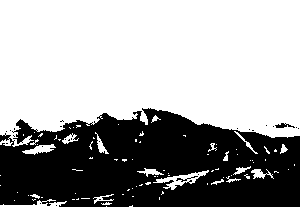
\includegraphics[width=\textwidth]{img/basics-image-binary}
    \caption{Obraz jednokanałowy(binarny)}
    \label{fig:basics_image_binary}
  \end{subfigure}
  \caption{Rodzaje obrazów cyfrowych}\label{fig:image_examples}
\end{figure}
\subsection{Podstawowe algorytmy przetwarzania obrazów}
\subsubsection{Kadrowanie obrazu}
Operacja kadrowania polega na pozostawieniu na obrazie wejściowym tylko tych pikseli, które znajdują się w zadanym, prostokątnym obszarze:
\begin{gather*}
  \forall p \in I\quad p.x \in {p1.x, p2.x} \wedge p.y \in {p1.y, p2.y}
\end{gather*}, gdzie:
\begin{itemize}
\item I - obraz wejściowy
\item p1 - współrzędne lewego górnego rogu obszaru kadru,
\item p2 - współrzędne prawego dolnego rogu obszaru kadru
\end{itemize}. Na rysunku ~\ref{fig:crop_image} przedstawiona została operacja kadrowania obrazu. Celem kadrowania jest usunięcie z obrazu informacji, które są zbędne podczas wykonywania analizy obrazu, ponieważ mogą negatywnie wpłynąć na czas oraz rezultaty wykonania algorytmów.
\begin{figure}
  \centering
  \begin{subfigure}[b]{0.45\textwidth}
    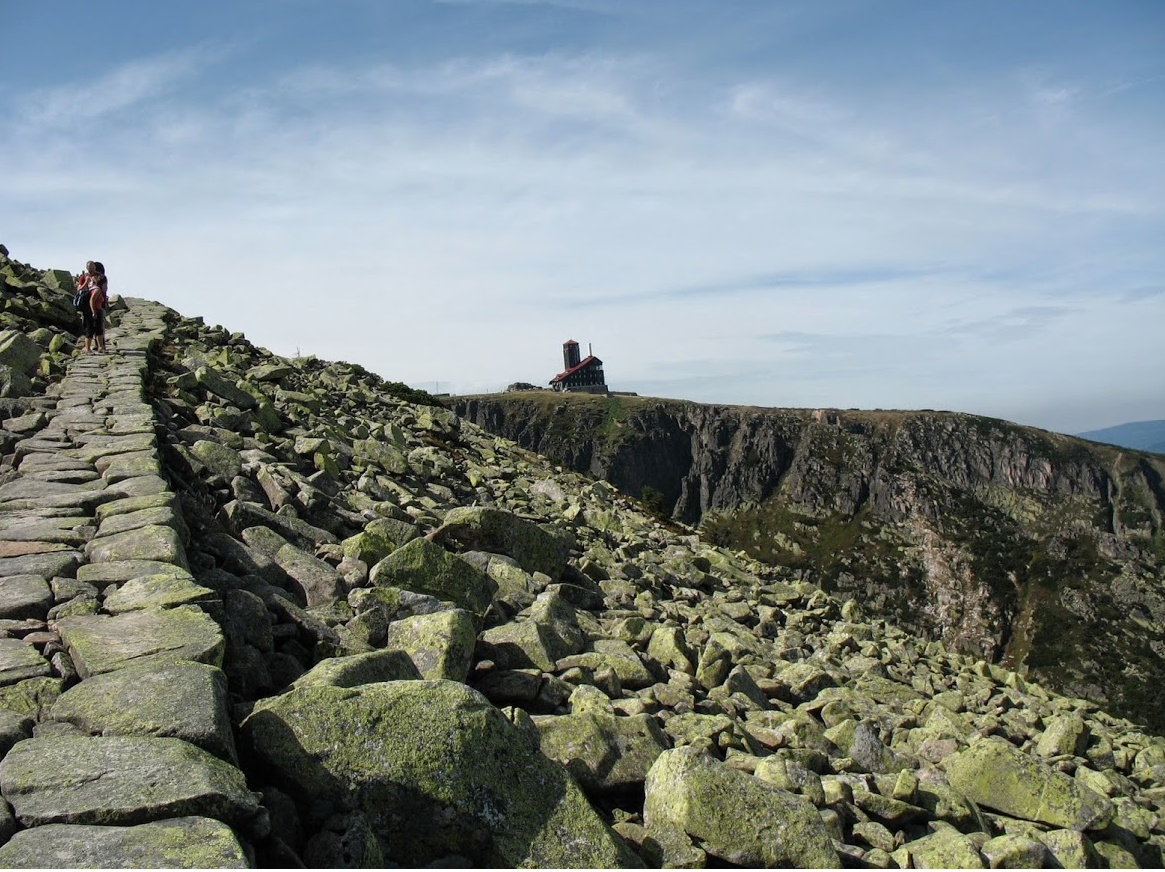
\includegraphics[width=\textwidth]{img/crop-image-before}
    \caption{Obraz wejściowy dla operacji kadrowania}
    \label{fig:crop_image_before}
  \end{subfigure}
  ~
  \begin{subfigure}[b]{0.45\textwidth}
    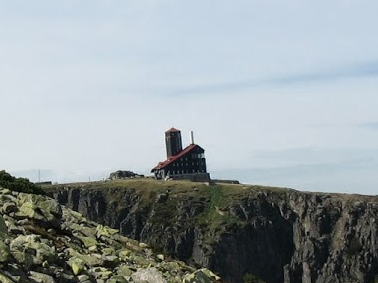
\includegraphics[width=\textwidth]{img/crop-image-after}
    \caption{Obraz wyjściowy, poddany operacji kadrowania}
    \label{fig:crop_image_after}
  \end{subfigure}
  \caption{Operacja kadrowania obrazu}\label{fig:crop_image}
\end{figure}
\subsubsection{Progowanie} \label{sssec:threshold}
Progowanie polega na podziale pikseli obrazu na dwie grupy, poprzez wybranie określonej wartości progowej $t$. Każdy piksel jest porównywany z wartością progową, i w zależności od tego, czy wartość piksela jest większa od wartości progowej, czy mniejsza, w tej samej pozycji nowo powstałego obrazu, przypisuje się wartość $1$, lub $0$. Operację można opisać wzorem:
\begin{gather*}
  I_{out}(x, y) = \left\{\begin{matrix}
  1, dla \: I_{in}(x, y) > t\\
  0, dla \: I_{in}(x, y) \leq t
  \end{matrix}\right. x=0,1,2,...,N-1; y=0,1,2,...,M-1
\end{gather*},
gdzie:
\begin{itemize}
\item $I_{in}$ - obraz wejściowy
\item $I_{out}$ - obraz wyjściowy
\item $N$ - szerokość obrazu
\item $M$ - wysokość obrazu
\end{itemize}
Na rysunku ~\ref{fig:threshold_image} przedstawiony został wynik operacji progowania na przykładowym obrazie monochromatycznym.
\begin{figure}
  \centering
  \begin{subfigure}[b]{0.45\textwidth}
    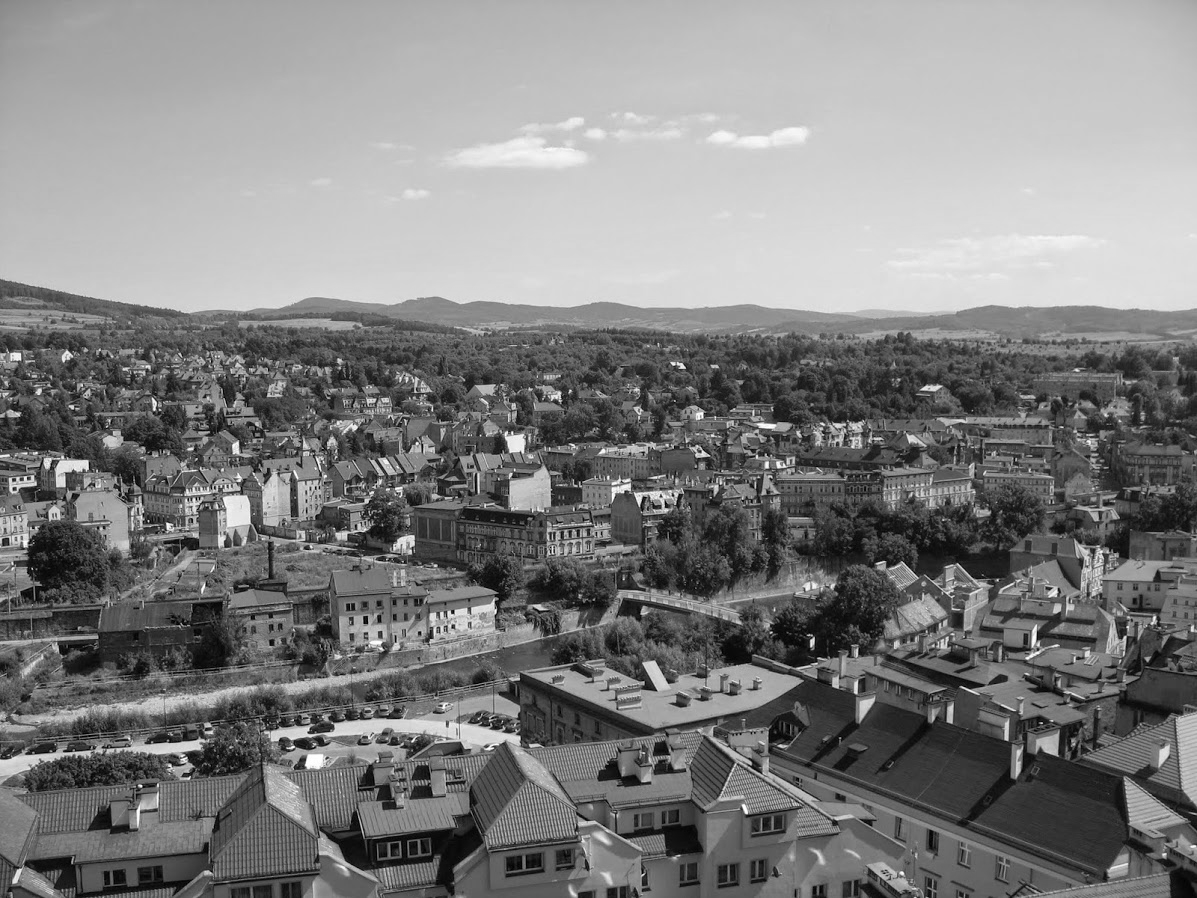
\includegraphics[width=\textwidth]{img/threshold-before}
    \caption{Obraz wejściowy dla operacji progowania}
    \label{fig:threshold_before}
  \end{subfigure}
  ~
  \begin{subfigure}[b]{0.45\textwidth}
    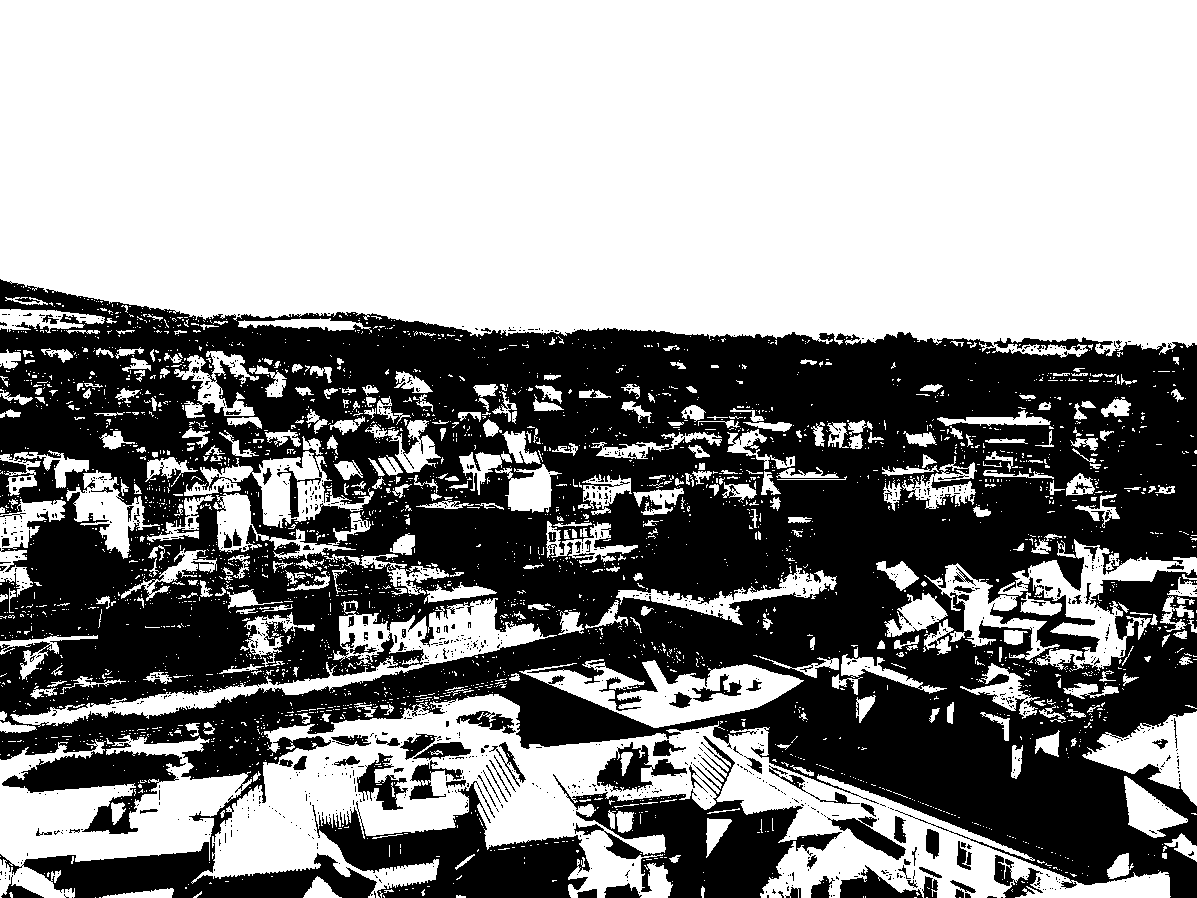
\includegraphics[width=\textwidth]{img/threshold-after}
    \caption{Obraz wyjściowy, poddany operacji progowania}
    \label{fig:threshold_after}
  \end{subfigure}
  \caption{Operacja progowania z wartością progu $t=128$ dla obrazu jednokanałowego}\label{fig:threshold_image}
\end{figure}

\paragraph{Progowanie obrazów z większą ilością składowych}\mbox{}\\
Zazwyczaj operacji progowania poddawane są obrazy jednokanałowe. Istnieje jednak możliwość wykonania operacji progowania dla obrazów wielokanałowych (np. dla obrazów RGB). Operacja ta definiowana jest następującym wzorem:
\begin{gather*}
  I_{out}(x, y) = \left\{\begin{matrix}
  1, \; \text{jeżeli} \; \forall c \in C, \; I_{in}(x, y, c) > t(c)\\
  0, \; \text{jeżeli} \; \exists c \in C, \; I_{in}(x, y, c) \leq t(c)
  \end{matrix}\right.\\ x=0,1,2,...,N-1; y=0,1,2,...,M-1; c=0,1,2,...,C
\end{gather*},
gdzie $C$ to liczba kanałów w obrazie.
Algorytm progowania operujący na wielu kanałach może zostać wykorzystany, kiedy znana jest dokładna barwa badanego obiektu.

\subsubsection{Filtracja obrazu}
Algorytmy filtracji mają na celu wykonanie zadanego przekształcenia matematycznego dla każdego piksela, generując tym samym nowy obraz. Filtrację obrazu stosuje się zwykle w celu wydobycia z obrazu żądanych informacji lub usunięcia szumu na obrazie. Poniżej wymienionych zostało kilka najczęściej używanych operacji filtrowania obrazu:
\begin{itemize}
\item filtr uśredniający - stosowany jest w celu rozmycia obrazu
  \begin{gather*}
    I_{out} = \frac{\sum_{x=M-k_x/2}^{M+k_x/2} \sum_{y=N-k_y/2}^{N+k_y/2} I_{in}(x, y)}{k_x*k_y}
  \end{gather*}, gdzie:
  \begin{itemize}
    \item M, N - rozmiar obrazu
    \item $k_x, k_y$ - rozmiar jądra użytego w algorytmie filtracji
    \item $I_{in}$ - obraz wejściowy
    \item $I_{out}$ - obraz wyjściowy
  \end{itemize}
\item filtr medianowy - wykorzystywany jest do usuwania zakłóceń na obrazie
  \begin{gather*}
    I_{out}(x, y) = median\_element(\{I_{in}(x, y), \;x \in <M-\frac{k_x}{2}, M+\frac{k_x}{2}> \\
    \vee\; y \in <N-\frac{k_y}{2}, N+\frac{k_y,}{2}>\})
    \end{gather*}
  \begin{itemize}
    \item M, N - rozmiar obrazu
    \item $k_x, k_y$ - rozmiar jądra użytego w algorytmie filtracji
    \item $I_{in}$ - obraz wejściowy
    \item $I_{out}$ - obraz wyjściowy
  \end{itemize}
\item filtr Gaussa - podobnie jak filtr uśredniający, filtr Gaussa stosuje się do redukcji detali na obrazie poprzez jego rozmycie
  \begin{gather*}
    I_{out}(x, y) = \frac{1}{\sqrt{2 \pi \sigma}} e^{-\frac{x^2}{2 \sigma^2}}
  \end{gather*}
\end{itemize}
. 
Rysunek~\ref{fig:lena_smooth} przedstawia zaszumiony obraz oraz wynik działania algorytmu rozmycia medianowego.
\begin{figure}
  \centering
  \begin{subfigure}[b]{0.45\textwidth}
    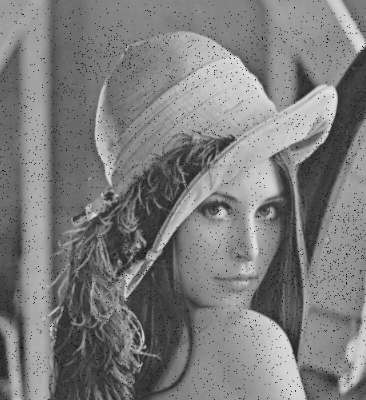
\includegraphics[width=\textwidth]{img/smooth-lena-input}
    \caption{Obraz wejściowy}
    \label{fig:smooth_lena_input}
  \end{subfigure}
  ~
  \begin{subfigure}[b]{0.45\textwidth}
    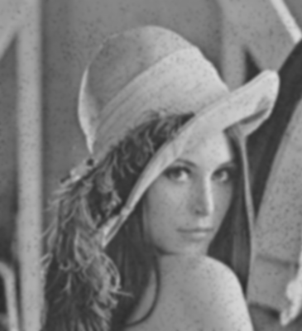
\includegraphics[width=\textwidth]{img/smooth-lena-gauss}
    \caption{Operacja rozmycia Gaussa}
    \label{fig:smooth_lena_gauss}
  \end{subfigure}
  ~
  \begin{subfigure}[b]{0.45\textwidth}
    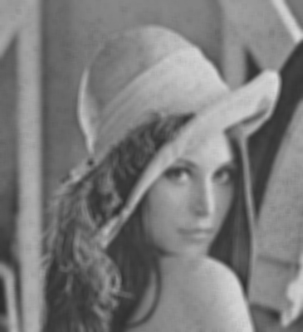
\includegraphics[width=\textwidth]{img/smooth-lena-mean}
    \caption{Operacja rozmycia średniego}
    \label{fig:smooth_lena_gauss}
  \end{subfigure}
  ~
  \begin{subfigure}[b]{0.45\textwidth}
    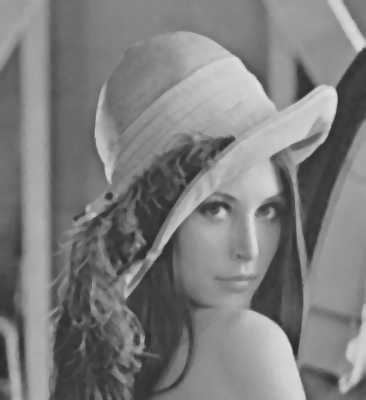
\includegraphics[width=\textwidth]{img/smooth-lena-median}
    \caption{Operacja rozmycia medianowego}
    \label{fig:smooth_lena_gauss}
  \end{subfigure}
  \caption{Wynik działania podstawowych operacji rozmycia na obrazie wejściowym}
  \label{fig:lena_smooth}
\end{figure}
\subsubsection{Dodawanie obrazów}
Operacja dodawania obrazów definiowana jest następująco:
\begin{gather*}
  I_{out}(x, y) = \displaystyle\sum_{i}^{C} I_i(x, y), \quad x \in <0; M>,  y \in <0; N>
\end{gather*}, gdzie:
\begin{itemize}
  \item C - liczba obrazów do posumowania
  \item $I_i$ - obrazy wejściowe, które zostaną dodane
  \item $I_{out}$ - obraz wyjściowy
  \item M, N - rozmiar obrazu wyjściowego
\end{itemize}
\paragraph{Dodawanie obrazów z wagami} \mbox{}\\
Dodawanie obrazów z wagami zdefiniowane jest wzorem:
\begin{gather*}
  I_{out}(x, y) = \displaystyle\sum_{i}^{C} I_i(x, y) * w_i, \quad x \in <0; M>, y \in <0; N>
\end{gather*}, gdzie:
\begin{itemize}
  \item $w_i$ - wektor wag dla poszczególnych obrazów wejściowych
  \end{itemize}.
\subsubsection{Wyostrzenie obrazu}
W celu uzyskania efektu wyostrzonych krawędzi obrazu, należy wykonać na obrazie wejściowym operację rozmycia Gaussa, a następnie obraz wynikowy dodać do obrazu wejściowego z wagami:
\begin{itemize}
  \item 1.5 dla obrazu wejściowego
  \item -0.5 dla obrazu poddanego operacji rozmycia Gaussa
\end{itemize}. Na rysunku~\ref{fig:image_sharpen} przedstawiono obraz poddany operacji wyostrzania, oraz wynik tej operacji.
\begin{figure}
  \centering
  \begin{subfigure}[b]{0.45\textwidth}
    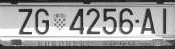
\includegraphics[width=\textwidth]{img/image-sharpen-before}
    \label{fig:image_sharpen_before}
  \end{subfigure}
  ~
  \begin{subfigure}[b]{0.45\textwidth}
    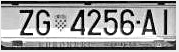
\includegraphics[width=\textwidth]{img/image-sharpen-after}
    \label{fig:image_sharpen_after}
  \end{subfigure}
  \caption{Operacja wyostrzenia wykonana na obrazie jednokanałowym}
  \label{fig:image_sharpen}
\end{figure}
\subsubsection{Normalizacja obrazu}
Operacja normalizacji służy do zmiany przedziału wartości pikseli występujących w obrazie. Algorytm można zapisać wzorem:
\begin{gather*}
  I_{out}(x, y) = (I_{in} - min_{in})*\frac{max_{out} - min_{out}}{max_{in} - min_{in}}+min_{in}, \quad x \in <0; M>,  y \in <0; N>
\end{gather*}, gdzie:
\begin{itemize}
\item $I_{in}$, $I_{out}$ - funkcja obrazu wejściowego i wyjściowego
\item $min_{in}$, $max_{in}$ - wartość minimalna i maksymalna na obrazie wejściowym
\item $min_{out}$, $max_{out}$ - żądana wartość minimalna i maksymalna dla obrazu wyjściowego
\item M, N - szerokość oraz wysokość obrazu
\end{itemize}
. Rysunek~\ref{fig:image_normalize} prezentuje działanie algorytmu normalizacji. Obraz wejściowy został wykonany w bardzo ciemnym otoczeniu, natomiast po wykonaniu operacji kontrast obrazu został poprawiony.
\begin{figure}
  \centering
  \begin{subfigure}[b]{0.45\textwidth}
    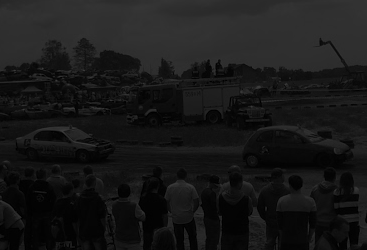
\includegraphics[width=\textwidth]{img/image-normalize-before}
    \label{fig:image_normalize_before}
  \end{subfigure}
  ~
  \begin{subfigure}[b]{0.45\textwidth}
    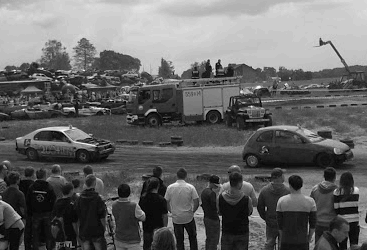
\includegraphics[width=\textwidth]{img/image-normalize-after}
    \label{fig:image_normalize_after}
  \end{subfigure}
  \caption{Normalizacja obrazu}
  \label{fig:image_normalize}
\end{figure}
\subsection{Operacje morfologiczne}
Operacje morfologiczne na obrazach wykorzystywane są do filtracji morfologicznej oraz analizy kształtów obiektów na obrazie. Algorytmy morfologiczne są podstawą dla wielu bardziej złożonych algorytmów analizy wizji komputerowej.
\subsubsection{Dylatacja obrazu}
Dylatacja to rozszerzenie obrazu wykorzystując zadany element strukturalny. Operacja definiowana jest wzorem
\begin{gather*}
  A \oplus B \equiv \bigcup \limits_{b \in B} A_b
\end{gather*}.
Przykładowy wynik operacji dylatacji przedstawiony jest na rysunku~\ref{fig:dilate}.
\begin{figure}
  \centering
  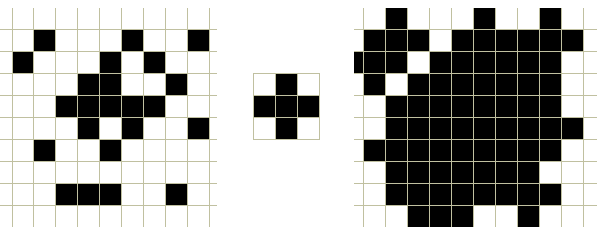
\includegraphics[width=15cm]{img/dilate}
  \caption{Obraz binarny poddany procesowi dylatacji z zadanym elementem strukturalnym}
  \label{fig:dilate}
\end{figure}
\subsubsection{Erozja obrazu} 
Erozja obrazu polega na zwężaniu obrazu z wykorzystaniem zadanego elementu strukturalnego. Operacja definiowana jest wzorem
\begin{gather*}
  A \ominus B \equiv \bigcap \limits_{b \in B} A_{-b}
\end{gather*}.
Przykładowy wynik operacji erozji obrazu przedstawiony został na rysunku~\ref{fig:erode}.
\begin{figure}
  \centering
  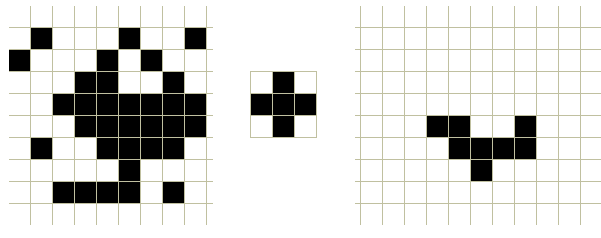
\includegraphics[width=15cm]{img/erode}
  \caption{Obraz binarny poddany procesowi erozji z zadanym elementem strukturalnym}
  \label{fig:erode}
\end{figure}
\subsubsection{Zamknięcie i otwarcie obrazu}
Operacje zamknięcia i otwarcia obrazu to złożenie dwóch wyżej wymienionych operacji (dylatacji oraz erozji) w odpowiedni sposób.
\begin{itemize}
\item zamknięcie obrazu definiowane jest w następujący sposób:
  \begin{gather*}
    A \bullet B = (A \oplus B) \ominus B
  \end{gather*}, czyli najpierw wykonywana jest operacja dylatacji obrazu, a następnie przekształcony obraz poddawany jest operacji erozji
\item otwarcie obrazu definiowane jest wzorem:
  \begin{gather*}
    A \circ B = (A \ominus B) \oplus B
  \end{gather*}. W przypadku algorytmu otwarcia obrazu, w pierwszej kolejności wykonywana jest operacja erozji, a następnie operacja dylatacji obrazu.
\end{itemize}
Na rysunku~\ref{fig:open_close} przedstawiony został wynik działania obydwu algorytmów na tym samym obrazie, z tym samym elementem strukturalnym.
\begin{figure}
  \centering
  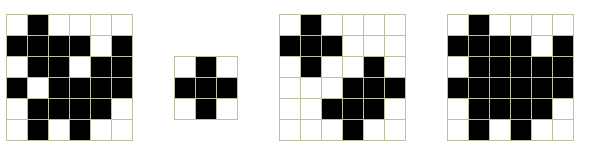
\includegraphics[width=15cm]{img/open-close}
  \caption{Obraz binarny poddany operacji otwarcia oraz zamknięcia obrazu, dla takiego samego elementu strukturalnego}
  \label{fig:open_close}
\end{figure}
\subsubsection{Transformata odległościowa}
Transformata odległościowa, inaczej zwana funkcją odległości, służy do wyznaczania minimalnej odległości punktu o wartości 1 od punktu o wartości 0. Dla punktów o wartości 0 automatycznie przypisywana jest wartość 0. \\
Tabela~\ref{tab:distance_transform} przedstawia wynik działania operacji na macierzy zawierającej obrazy binarne, natomiast rysunek~\ref{fig:distance_transform} prezentuje wynik działania tej samej operacji na obrazie. W celu podkreślenia wyniku operacji, obraz wyjściowy został poddany operacji normalizacji.

\begin{table}
\centering
\begin{minipage}[b]{80mm}
\centering
\begin{tabular}{|l|l|l|l|l|l|l|l|}
\hline
0&0&0&0&0&0&0&0 \\ \hline
0&1&1&1&1&1&1&0 \\ \hline
0&1&1&1&1&1&1&0 \\ \hline
0&1&1&1&1&1&1&0 \\ \hline
0&1&1&1&1&1&1&0 \\ \hline
0&1&1&1&1&1&1&0 \\ \hline
0&0&0&0&0&0&0&0 \\ \hline
\end{tabular}
\caption*{Binarny obraz wejściowy}
\end{minipage}
\begin{minipage}[b]{70mm}
\centering
\begin{tabular}{|l|l|l|l|l|l|l|l|}
\hline
0&0&0&0&0&0&0&0 \\ \hline
0&1&1&1&1&1&1&0 \\ \hline
0&1&2&2&2&2&1&0 \\ \hline
0&1&2&3&3&2&1&0 \\ \hline
0&1&2&2&2&2&1&0 \\ \hline
0&1&1&1&1&1&1&0 \\ \hline
0&0&0&0&0&0&0&0 \\ \hline
\end{tabular}
\caption*{Transformata odległościowa}
\end{minipage}
\caption{Transformacja odległościowa - macierz binarna} \label{tab:distance_transform} 
\end{table}

\begin{figure}
  \centering
  \begin{subfigure}[b]{0.45\textwidth}
    
\includegraphics[width=\textwidth]{img/distance-transform-before}
    \caption{Binarny obraz wejściowy}
    \label{fig:distance_transform_before}
  \end{subfigure}
  ~
  \begin{subfigure}[b]{0.45\textwidth}
    
\includegraphics[width=\textwidth]{img/distance-transform-after}
    \caption{Transformata odległościowa}
    \label{fig:distance_transform_after}
  \end{subfigure}
    \caption{Transformacja odległościowa - obraz binarny}
    \label{fig:distance_transform}
\end{figure}

\subsection{Operacje na histogramach}
Bardzo często podczas analizy obrazu pod kątem znajdowania segmentów, wykorzystywana jest analiza histogramu. W celu ułatwienia analizy, a także poprawy jej wyników, przed jej rozpoczęciem można zastosować niżej wymienione algorytmy.
\subsubsection{Histogram obrazu}
\begin{figure}
  \centering
  \begin{subfigure}[b]{0.45\textwidth}
    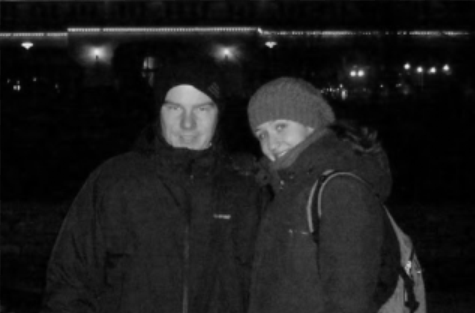
\includegraphics[width=\textwidth]{img/image-histogram}
    \label{fig:image_histogram}
  \end{subfigure}
  ~
  \begin{subfigure}[b]{0.45\textwidth}
    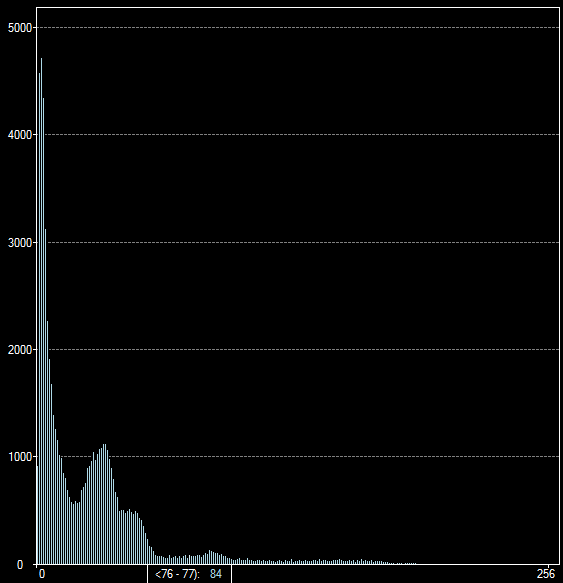
\includegraphics[width=\textwidth]{img/image-histogram-histogram}
    \label{fig:image_histogram_histogram}
  \end{subfigure}
  \caption{Jednokanałowy obraz oraz jego histogram}
  \label{fig:image_histogram_g}
\end{figure}
Histogram obrazu jest graficzną reprezentacją rozkładu częstości występowania danej wartości jasności w obrazie. Przykładowy obraz oraz jego histogram przedstawiony został na rysunku~\ref{fig:image_histogram_g}. Ponieważ obraz jest bardzo ciemny, większość wartości na histogramie jest bliska wartości 0(ta wartość reprezentuje kolor czarny).
\subsubsection{Wyrównanie histogramu}
Metoda wyrównywania histogramu ma na celu zmianę kontrastu obrazu. Algorytm wykorzystywany jest w przypadku, gdy zarówno tło, jak i pierwszy plan obrazu, są ciemne lub jasne. Wadą metody wyrównywania histogramu jest możliwe wzmocnienie zakłóceń występujących na obrazie, gdyż algorytm traktuje je jak sygnał opisujący prawidłowy obraz. Przed zastosowaniem tej metody, warto zatem zastosować jeden z algorytmów rozmycia obrazu, opisywany we wcześniejszej części tego rozdziału.\\
Metoda wyrównania histogramu sprowadza się do wyznaczenia tablicy LUT(\textit{ang. Lookup table}), na podstawie której wyznaczone zostaną wartości poszczególnych pikseli obrazu wejściowego. W celu wyznaczenia tablicy LUT, należy wyznaczyć dystrybuantę rozkładu prawdopodobieństwa dla wartości pikseli obrazu:
\begin{gather*}
  D(i) = \sum\limits_{j=0}^i p(j)
\end{gather*}, gdzie i jest wartością występującą na obrazie, a p(j) jest prawdopodobieństwem wystąpienia wartości j w obrazie. Wykorzystując wyznaczone wartości dystrybuanty, możemy opisać tablicę LUT za pomocą wzoru:
\begin{gather*}
  LUT(i) = \frac{D(i)-D_0}{1-D_0}*K
\end{gather*}, gdzie i to wartość składowej obrazu wejściowego, $D_0$ to pierwsza wartość dystrybuanty różna od zera, a K jest maksymalną wartością występującym w obrazie wejściowym.\\
Rysunek~\ref{fig:equalize_histogram} przedstawia efekt działania operacji wyrównania histogramu na przykładowym obrazie.
\begin{figure}
  \centering
  \begin{subfigure}[b]{0.45\textwidth}
    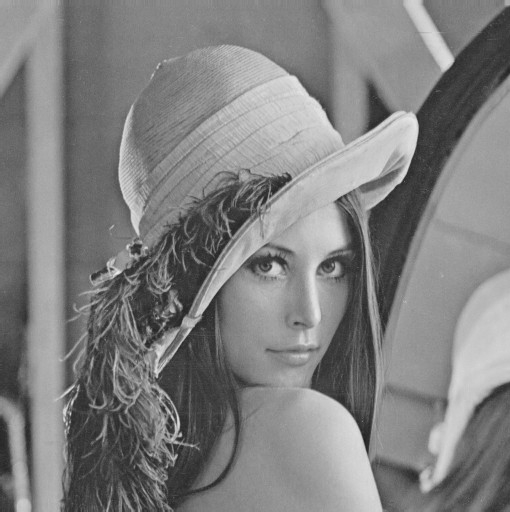
\includegraphics[width=\textwidth]{img/equalize-histogram-before}
    \caption{Obraz wejściowy dla operacji wyrównania histogramu}
    \label{fig:equalize_histogram_before}
  \end{subfigure}
  ~
  \begin{subfigure}[b]{0.45\textwidth}
    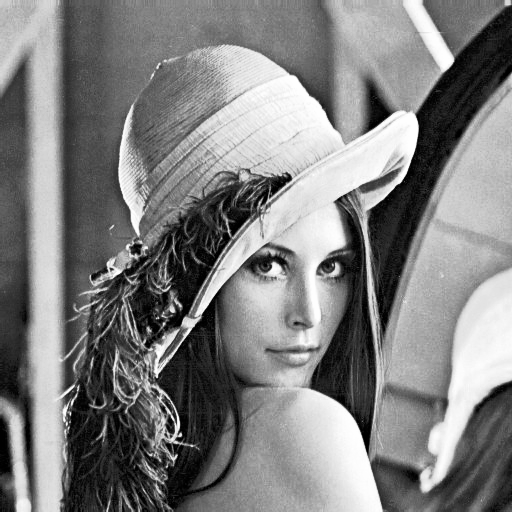
\includegraphics[width=\textwidth]{img/equalize-histogram-after}
    \caption{Obraz wyjściowy, poddany operacji wyrównania histogramu}
    \label{fig:equalize_histogram_after}
  \end{subfigure}
  ~
  \begin{subfigure}[b]{0.45\textwidth}
    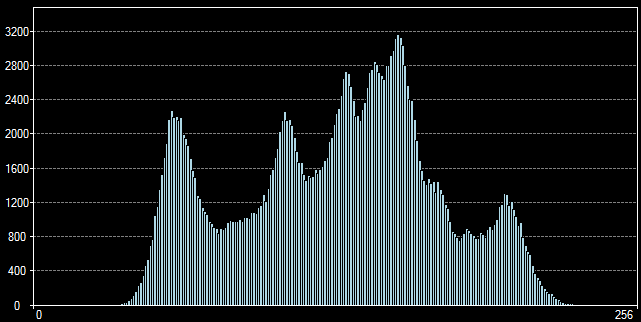
\includegraphics[width=\textwidth]{img/equalize-histogram-histogram-before}
    \caption{Histogram obrazu wejściowego}
    \label{fig:equalize_histogram_histogram_before}
  \end{subfigure}
  ~
  \begin{subfigure}[b]{0.45\textwidth}
    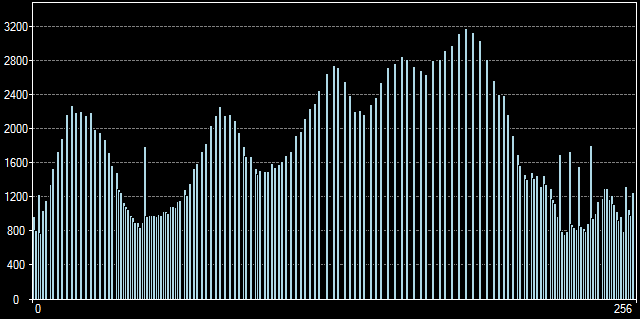
\includegraphics[width=\textwidth]{img/equalize-histogram-histogram-after}
    \caption{Histogram obrazu wyjściowego}
    \label{fig:equalize_histogram_histogram_after}
  \end{subfigure}
  \caption{Operacja wyrównania histogramu dla obrazu jednokanałowego}\label{fig:equalize_histogram}
\end{figure}

\subsubsection{Wygładzenie histogramu}
Często histogram obrazu zawiera w sobie nagłe skoki wartości, które utrudniają analizę histogramu, gdyż mogą reprezentować fałszywe ekstrema. Wygładzanie histogramu ma na celu usunięcie takich skoków, zachowując przy tym oryginalny kształt histogramu. Dla każdej wartości histogramu wejściowego \textit{$H_{in}$} należy zastosować następującą operację:
\begin{gather*}
  \vee i \in <H_{in}(0), H_{in}(H_{max})> H_{out}(i) = H_{in}(i-1) + H_{in}(i) + H_{in}(i+1)
\end{gather*},
gdzie \textit{$H_{out}$} jest histogramem wyjściowym, a $H_{max}$ największym indeksem w histogramie. Przykład działania algorytmu wygładzania histogramu przedstawiony został na rysunku~\ref{fig:histogram_smooth}
\begin{figure}
  \centering
  \begin{subfigure}[b]{0.45\textwidth}
    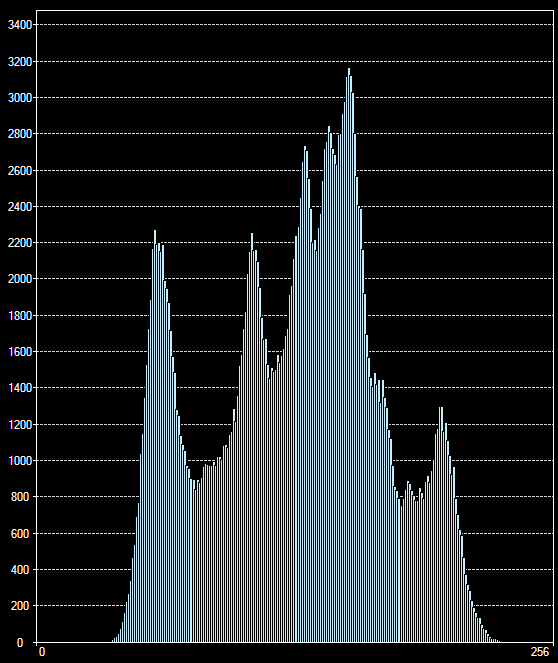
\includegraphics[width=\textwidth]{img/smooth-histogram-before}
    \caption{Obraz wejściowy dla operacji wygładzenia histogramu}
    \label{fig:equalize_histogram_before}
  \end{subfigure}
  ~
  \begin{subfigure}[b]{0.45\textwidth}
    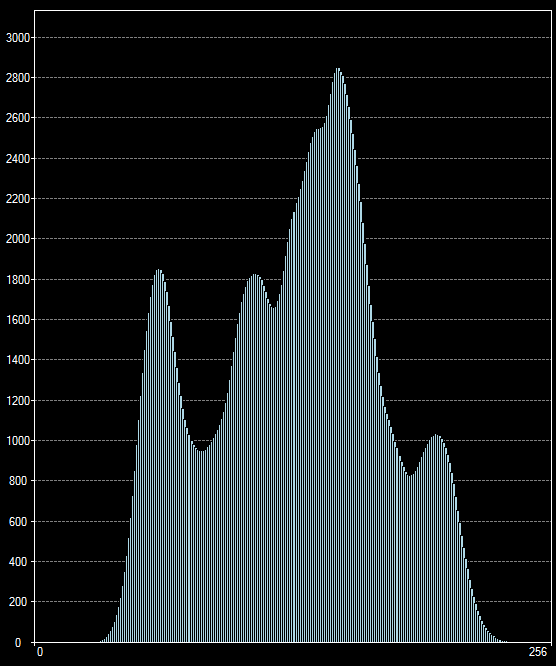
\includegraphics[width=\textwidth]{img/smooth-histogram-after}
    \caption{Obraz wyjściowy, poddany operacji wygładzenia histogramu}
    \label{fig:equalize_histogram_after}
  \end{subfigure}
  \caption{Operacja wygładzenia histogramu}\label{fig:histogram_smooth}
\end{figure}
